\documentclass[11pt]{article}
\usepackage[utf8]{inputenc}
\usepackage[T1]{fontenc}
\usepackage{geometry, tikz, xcolor, enumitem, ragged2e}
\geometry{a4paper, margin=1.5cm}

\begin{document}

\begin{center}
\Large \textbf{\textcolor{blue!60!black}{Atividade Remota: Matemática – Análise Combinatória}}\\[0.3cm]
\large Professor: Jefferson
\end{center}

\vspace{0.3cm}
\large Nome: \underline{\hspace{8cm}} \quad Turma: \underline{\hspace{3cm}}

\vspace{0.5cm}

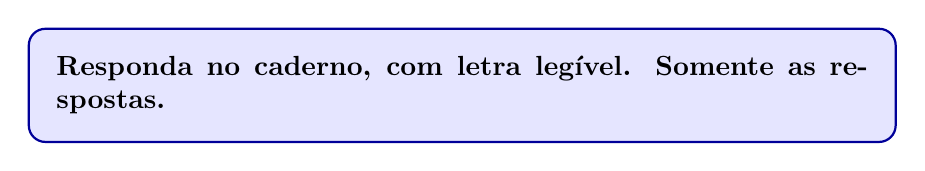
\begin{tikzpicture}
\node[rectangle, fill=blue!10, rounded corners=6pt, inner sep=10pt, draw=blue!60!black, thick]{
\begin{minipage}{0.85\linewidth}
\textbf{Responda no caderno, com letra legível. Somente as respostas.}
\end{minipage}
};
\end{tikzpicture}

\vspace{0.6cm}

\begin{enumerate}
\item Explique com suas palavras o que é o \textbf{princípio fundamental da contagem} e dê um exemplo prático.\\[1em]
\rule{\linewidth}{0.4pt}\\[1em]\rule{\linewidth}{0.4pt}\\[1em]\rule{\linewidth}{0.4pt}\\[1em]\rule{\linewidth}{0.4pt}\\[1em]\rule{\linewidth}{0.4pt}\\[1em]\rule{\linewidth}{0.4pt}\\[1em]\rule{\linewidth}{0.4pt}\\[1em]\rule{\linewidth}{0.4pt}

\item O que diferencia uma \textbf{permutação} de um \textbf{arranjo}?\\[1em]
\rule{\linewidth}{0.4pt}\\[1em]\rule{\linewidth}{0.4pt}\\[1em]\rule{\linewidth}{0.4pt}\\[1em]\rule{\linewidth}{0.4pt}\\[1em]\rule{\linewidth}{0.4pt}\\[1em]\rule{\linewidth}{0.4pt}\\[1em]\rule{\linewidth}{0.4pt}\\[1em]\rule{\linewidth}{0.4pt}

\item Em que tipo de problema é mais adequado usar uma \textbf{combinação}?\\[1em]
\rule{\linewidth}{0.4pt}\\[1em]\rule{\linewidth}{0.4pt}\\[1em]\rule{\linewidth}{0.4pt}\\[1em]\rule{\linewidth}{0.4pt}\\[1em]\rule{\linewidth}{0.4pt}\\[1em]\rule{\linewidth}{0.4pt}\\[1em]\rule{\linewidth}{0.4pt}\\[1em]\rule{\linewidth}{0.4pt}

\item Dê um exemplo de situação cotidiana que envolva uma escolha com \textbf{ordem relevante}.\\[1em]
\rule{\linewidth}{0.4pt}\\[1em]\rule{\linewidth}{0.4pt}\\[1em]\rule{\linewidth}{0.4pt}\\[1em]\rule{\linewidth}{0.4pt}\\[1em]\rule{\linewidth}{0.4pt}\\[1em]\rule{\linewidth}{0.4pt}\\[1em]\rule{\linewidth}{0.4pt}\\[1em]\rule{\linewidth}{0.4pt}

\item Como o conceito de \textbf{fatorial} se relaciona com permutações?\\[1em]
\rule{\linewidth}{0.4pt}\\[1em]\rule{\linewidth}{0.4pt}\\[1em]\rule{\linewidth}{0.4pt}\\[1em]\rule{\linewidth}{0.4pt}\\[1em]\rule{\linewidth}{0.4pt}\\[1em]\rule{\linewidth}{0.4pt}\\[1em]\rule{\linewidth}{0.4pt}\\[1em]\rule{\linewidth}{0.4pt}

\item De que forma as combinações são aplicadas em sorteios e seleções?\\[1em]
\rule{\linewidth}{0.4pt}\\[1em]\rule{\linewidth}{0.4pt}\\[1em]\rule{\linewidth}{0.4pt}\\[1em]\rule{\linewidth}{0.4pt}\\[1em]\rule{\linewidth}{0.4pt}\\[1em]\rule{\linewidth}{0.4pt}\\[1em]\rule{\linewidth}{0.4pt}\\[1em]\rule{\linewidth}{0.4pt}

\item Por que a análise combinatória é importante para a estatística e probabilidade?\\[1em]
\rule{\linewidth}{0.4pt}\\[1em]\rule{\linewidth}{0.4pt}\\[1em]\rule{\linewidth}{0.4pt}\\[1em]\rule{\linewidth}{0.4pt}\\[1em]\rule{\linewidth}{0.4pt}\\[1em]\rule{\linewidth}{0.4pt}\\[1em]\rule{\linewidth}{0.4pt}\\[1em]\rule{\linewidth}{0.4pt}

\item Escolher 3 representantes entre 10 alunos é um exemplo de qual tipo de contagem? Justifique.\\[1em]
\rule{\linewidth}{0.4pt}\\[1em]\rule{\linewidth}{0.4pt}\\[1em]\rule{\linewidth}{0.4pt}\\[1em]\rule{\linewidth}{0.4pt}\\[1em]\rule{\linewidth}{0.4pt}\\[1em]\rule{\linewidth}{0.4pt}\\[1em]\rule{\linewidth}{0.4pt}\\[1em]\rule{\linewidth}{0.4pt}

\end{enumerate}

\end{document}

